\documentclass[twocolumn]{article}

\usepackage[utf8]{inputenc}
\usepackage[T1]{fontenc}
\usepackage[vietnamese]{babel}
\usepackage[margin=1.25in]{geometry}
\usepackage{authblk}
\usepackage{setspace}
\usepackage{graphicx}
\usepackage{subcaption}
\usepackage{amsmath}
\usepackage{booktabs}
\usepackage{array}
\usepackage{xcolor}
\usepackage{listings}
\usepackage{hyperref}
\usepackage{enumitem}

% Cấu hình hiển thị code
\lstset{
	basicstyle=\ttfamily\small,
	backgroundcolor=\color{gray!10},
	frame=single,
	breaklines=true,
	captionpos=b,
	numbers=left,
	numberstyle=\tiny\color{gray},
	keywordstyle=\color{blue},
	commentstyle=\color{green!50!black},
	stringstyle=\color{red!70!black}
}

\setlength{\columnsep}{24pt}
\usepackage[switch]{lineno}
\setlength\linenumbersep{8pt}

%%%%%% Bibliography %%%%%%
\usepackage[style=nejm, citestyle=numeric-comp, sorting=none]{biblatex}
\addbibresource{sample.bib} 

%%%%%% Title & Authors %%%%%%
\title{\textbf{Triển khai Nền tảng Hybrid-Digital Twin Dựa trên Eclipse BaSyx: Từ Nghiên cứu đến Triển khai trên Server}}
\author[1,2]{Thái Đặng Phương Nam}
\author[2]{Nguyễn Lê Thanh Phong}
\author[2]{Huỳnh Thanh Sơn}
\affil[1]{Người báo cáo chính}
\affil[2]{Wisdom Software}
\affil[*]{TP. Hồ Chí Minh, Tháng 03 năm 2026}

\renewcommand\Authands{, }
\setstretch{1.15}

\begin{document}

\twocolumn[
	\begin{@twocolumnfalse}
		\maketitle
		\begin{abstract}
			Báo cáo này trình bày toàn diện quá trình nghiên cứu, triển khai và vận hành nền tảng Hybrid-Digital Twin (DT) dựa trên hệ sinh thái Eclipse BaSyx tại Wisdom Software. Dự án bao gồm ba giai đoạn chính: (1) Nghiên cứu ý tưởng số hóa thiết bị và quản lý thông số bằng công nghệ Digital Twin; (2) Triển khai thử nghiệm trên môi trường local với giao diện React, backend Docker, cơ sở dữ liệu MongoDB và middleware BaSyx DataBridge; (3) Triển khai lên server thực tế của công ty thông qua AnyDesk, bao gồm các bài thực hành deploy cơ bản và nghiên cứu chuyên sâu về kiến trúc Load Balancing, Container Orchestration nhằm chuẩn bị cho việc đưa dự án Digital Twin vào vận hành chuẩn trên server. Báo cáo tuân thủ nghiêm ngặt các tiêu chuẩn IEC 63278 và ISO 23247-2 trong thiết kế hệ thống.
		\end{abstract}
		\vspace{1.5em}
	\end{@twocolumnfalse}
]

%% ================================================================
%%  PHẦN 1: GIỚI THIỆU
%% ================================================================
\section{Giới thiệu}

\subsection{Bối cảnh và Động lực}
Trong bối cảnh cuộc Cách mạng Công nghiệp 4.0 đang diễn ra mạnh mẽ, việc tối ưu hóa quy trình sản xuất thông qua số hóa đã trở thành một yêu cầu cấp thiết. Dự án ``Hybrid-Digital Twin Platform'' được hình thành như một nỗ lực nghiên cứu và triển khai thực tiễn hệ thống bản sao số, tận dụng sức mạnh của hệ sinh thái mã nguồn mở Eclipse BaSyx. Mục tiêu cốt lõi của dự án không chỉ dừng lại ở việc xây dựng một giao diện Web UI đơn thuần để hiển thị dữ liệu, mà còn tập trung vào việc nghiên cứu sâu cơ chế vận hành của Asset Administration Shell (AAS) -- thành phần được coi là ``hộ chiếu kỹ thuật số'' cho các tài sản công nghiệp. Thông qua nền tảng này, nhóm thực hiện hướng tới việc thiết lập một hệ thống quản lý toàn diện, có khả năng theo dõi và điều phối vòng đời của tài sản từ giai đoạn cấu hình ban đầu đến quá trình vận hành thực tế tại nhà máy.

\subsection{Ý tưởng: Số hóa Thiết bị với Digital Twin}
Ý tưởng cốt lõi của dự án xuất phát từ nhu cầu \textbf{số hóa các thiết bị vật lý} và \textbf{quản lý các thông số hoạt động} của chúng một cách tập trung. Mô hình Digital Twin cho phép tạo ra một bản sao số (digital replica) của thiết bị thực, trong đó mọi thông số kỹ thuật, trạng thái vận hành và dữ liệu cảm biến đều được phản ánh theo thời gian thực. Cụ thể, quy trình số hóa bao gồm:

\begin{itemize}[noitemsep]
	\item \textbf{Định danh tài sản:} Mỗi thiết bị vật lý được gán một Asset Administration Shell (AAS) -- đóng vai trò như hộ chiếu kỹ thuật số chứa toàn bộ thông tin về thiết bị.
	\item \textbf{Mô hình hóa thông số:} Các thông số kỹ thuật (Technical Data), dữ liệu vận hành (Operational Data), tài liệu kỹ thuật (Documentation) được tổ chức dưới dạng Submodel theo tiêu chuẩn IEC 63278.
	\item \textbf{Kết nối thời gian thực:} Thông qua giao thức MQTT và BaSyx DataBridge, dữ liệu từ cảm biến vật lý được truyền liên tục đến bản sao số, cho phép giám sát và phân tích từ xa.
\end{itemize}

\subsection{Tiêu chuẩn hóa}
Về mặt tiêu chuẩn hóa, hệ thống được xây dựng để trở thành một hình mẫu về tính liên thông quốc tế bằng cách tuân thủ nghiêm ngặt tiêu chuẩn \textbf{IEC 63278}, đảm bảo cấu trúc của AAS được thống nhất và có thể hiểu được bởi các hệ thống khác nhau trong hệ sinh thái công nghiệp. Bên cạnh đó, việc áp dụng mô hình tham chiếu \textbf{ISO 23247-2} giúp dự án phân tách rõ ràng các dịch vụ quản lý tài nguyên số (Digital Twin Entity) và các thực thể giao tiếp thiết bị (Device Communication Entity). Sự kết hợp giữa các tiêu chuẩn này cung cấp một khung sườn vững chắc cho việc trao đổi thông tin an toàn, tin cậy và thúc đẩy khả năng tương tác giữa các hệ thống IT (Công nghệ thông tin) và OT (Công nghệ vận hành).

\subsection{Phạm vi Kỹ thuật}
Phạm vi kỹ thuật của dự án tập trung vào ba trụ cột chính: \textit{kết nối đồng bộ Frontend-Backend}, \textit{lưu trữ dữ liệu bền vững} và \textit{tích hợp dữ liệu thời gian thực}. Nhóm đã triển khai giải pháp kết nối giao diện người dùng dựa trên React với hệ thống Backend mạnh mẽ của BaSyx, cho phép quản lý các tập tin .aasx và cấu trúc Submodel một cách linh hoạt. Một điểm nhấn quan trọng là việc chuyển đổi từ lưu trữ tạm thời sang cơ chế lưu trữ bền vững với MongoDB Atlas, giúp loại bỏ hoàn toàn rủi ro mất mát dữ liệu khi hệ thống gặp sự cố hoặc tái khởi động. Cuối cùng, thông qua việc sử dụng BaSyx DataBridge, dự án thiết lập các luồng dữ liệu liên tục từ các cảm biến vật lý sử dụng giao thức MQTT đến bản sao số, cho phép cập nhật trạng thái thực tế của thiết bị lên môi trường ảo theo thời gian thực.

%% ================================================================
%%  PHẦN 2: KIẾN TRÚC VÀ TRIỂN KHAI (LOCAL)
%% ================================================================
\section{Kiến trúc và Triển khai trên Môi trường Local}
\subsection{Thành phần Hệ thống và Công nghệ}

\begin{figure*}[h!]
      \centering
      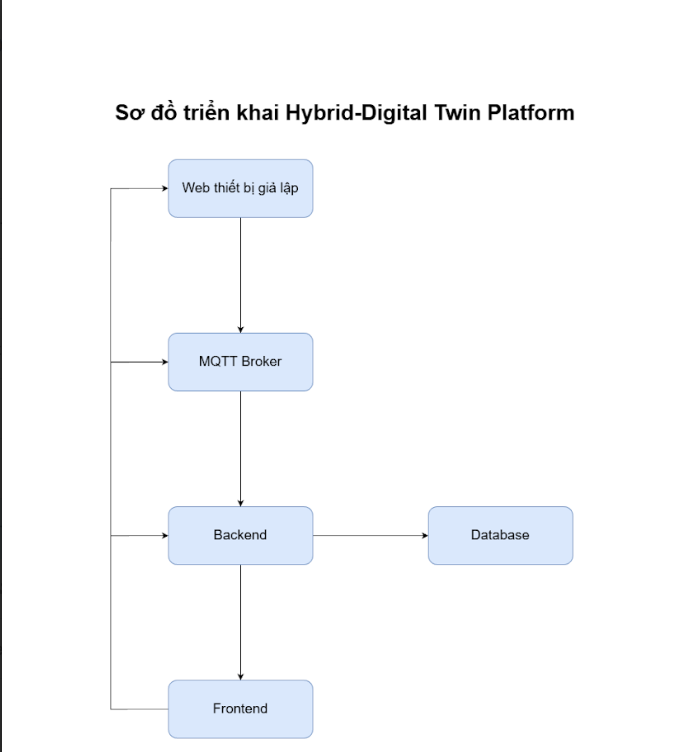
\includegraphics[width=\textwidth]{sodotrienkhai.png}
      \caption{Sơ đồ kiến trúc tổng thể của hệ thống Hybrid-Digital Twin Platform, bao gồm các thành phần Frontend, Backend, Cơ sở dữ liệu và Middleware.}
      \label{fig:sodotrienkhai}
\end{figure*}

\begin{itemize}
	\item \textbf{Frontend:} Thành phần giao diện người dùng được xây dựng bằng cách sử dụng mã nguồn chính thức từ hệ sinh thái Eclipse BaSyx, cụ thể là dự án \textit{basyx-aas-web-ui} dựa trên nền tảng React và Node.js. Quy trình triển khai bắt đầu bằng việc sao chép kho lưu trữ, sau đó thực hiện lệnh \texttt{npm install} để cài đặt các gói phụ thuộc cần thiết và khởi chạy môi trường phát triển thông qua lệnh \texttt{npm run dev}. Kết quả là một giao diện web trực quan hoạt động tại địa chỉ \texttt{localhost:3000}, cho phép người dùng tương tác với các bản sao số thông qua bố cục ba cột khoa học: cột bên trái hiển thị danh sách các AAS và hỗ trợ tải lên các tệp \texttt{.aasx}; cột giữa trình bày cấu trúc cây của các Submodel cùng các phần tử dữ liệu; và cột bên phải cung cấp thông tin chi tiết, hình ảnh hóa dữ liệu dưới dạng biểu đồ hoặc bảng, cùng với chế độ xem JSON dành cho lập trình viên.
  
  \begin{figure*}[h!]
      \centering
      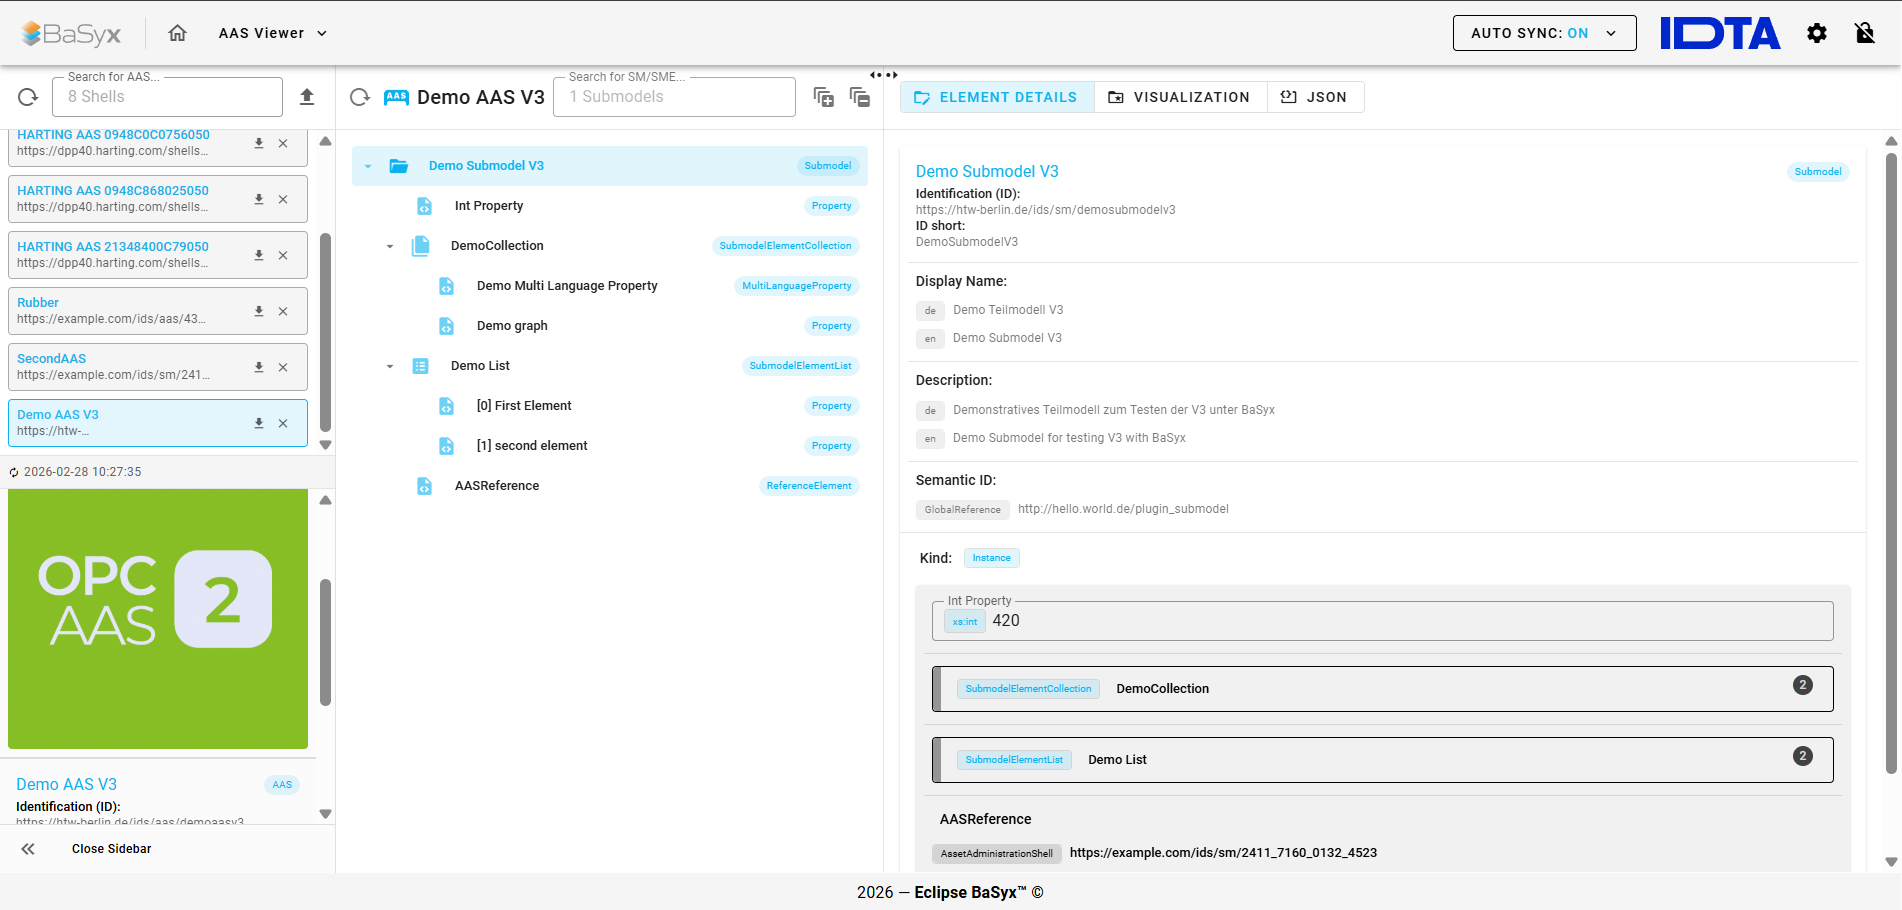
\includegraphics[width=\textwidth]{frontend.png}
      \caption{Giao diện Frontend của hệ thống Hybrid-Digital Twin Platform, cho phép người dùng tương tác với các bản sao số thông qua bố cục ba cột.}
      \label{fig:frontend}
  \end{figure*}

	\item \textbf{Backend:} Thay vì thiết lập thủ công các thành phần phức tạp của \textit{basyx-java-server-sdk}, hệ thống sử dụng giải pháp tối ưu hơn là triển khai thông qua Docker Compose với hình ảnh \texttt{aas-environment:2.0.0-milestone-08}. Container này, được đặt tên là \texttt{basyx-backend-service-ver1-0}, đóng vai trò là nhà cung cấp API RESTful cốt lõi tại cổng 8081, cho phép thực hiện toàn bộ các thao tác CRUD trên các vỏ quản trị tài sản và các mô hình con. Để đảm bảo tính tương tác mượt mà với Frontend chạy trên cổng 3000, các biến môi trường như \texttt{Basyx\_Cors\_Allowed-Origins=*} đã được cấu hình trong tệp \texttt{docker-compose.yml} nhằm khắc phục triệt để lỗi chặn tài nguyên từ nguồn khác (CORS). Ngoài ra, công cụ Swagger UI tại địa chỉ \texttt{localhost:8081/swagger-ui/index.html} cũng được tích hợp để hỗ trợ nhóm trong việc kiểm tra tính sẵn sàng và thử nghiệm trực tiếp các điểm cuối của API.
  
  \begin{figure*}[h!]
      \centering
      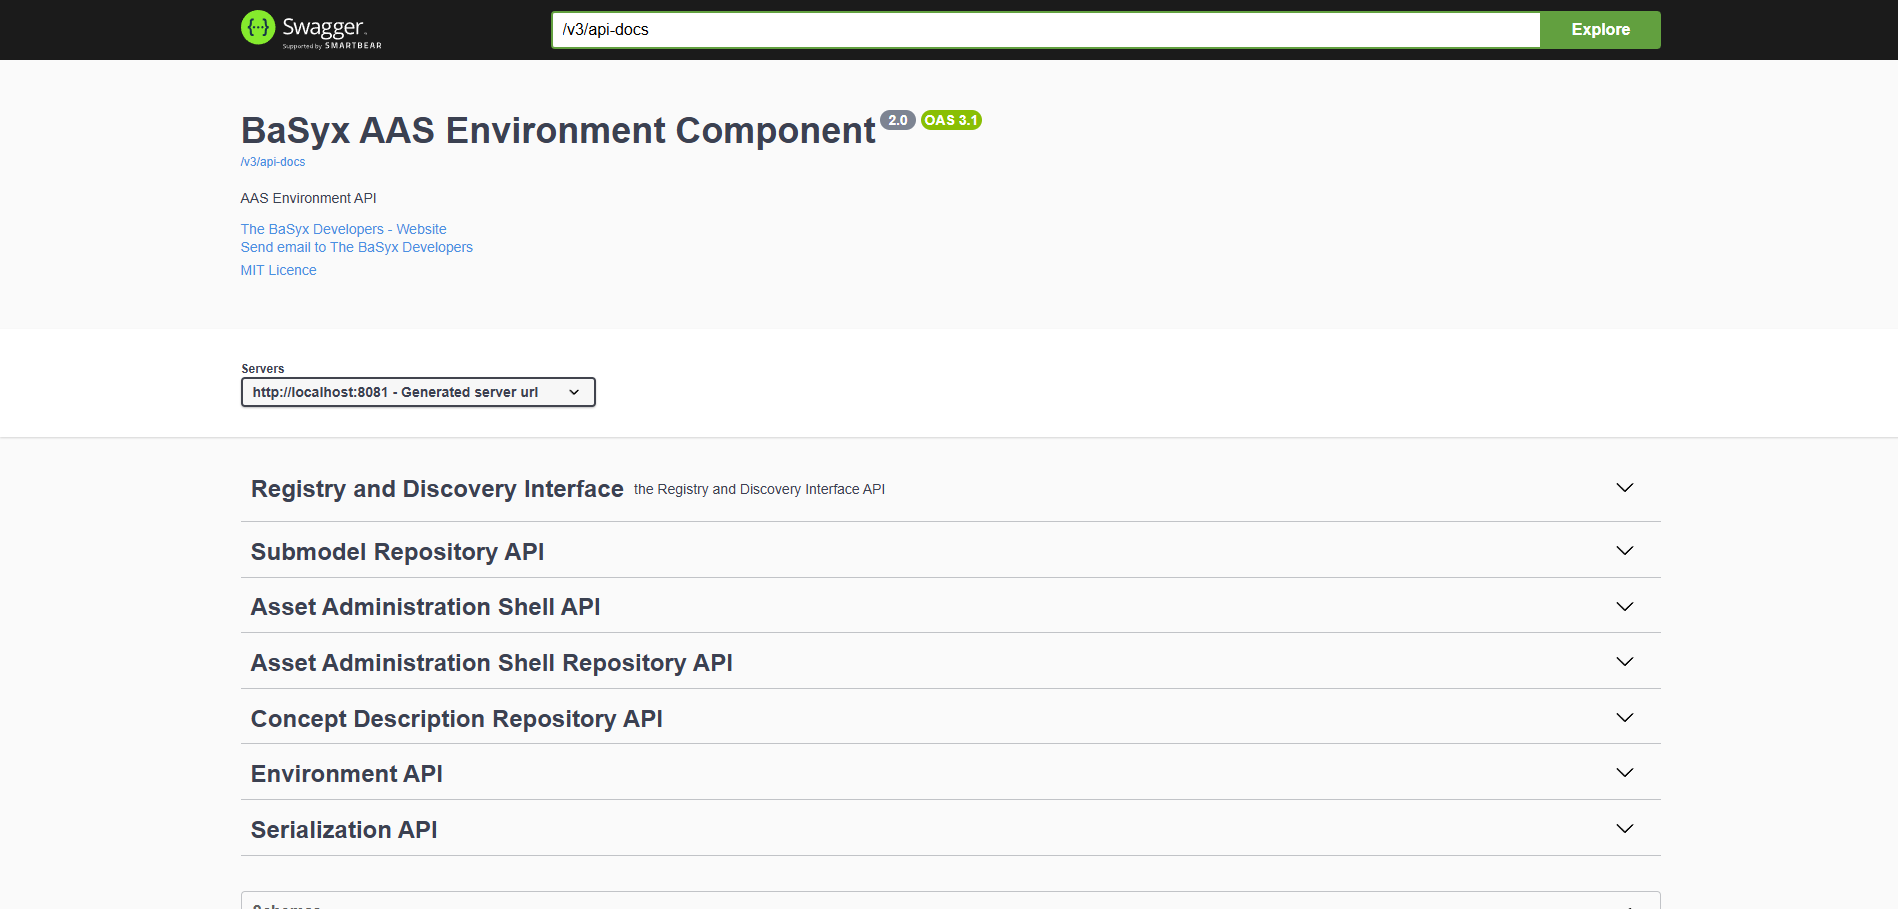
\includegraphics[width=\textwidth]{swagger.png}
      \caption{Giao diện Swagger UI hiển thị các endpoint API của BaSyx Backend Service.}
      \label{fig:swagger}
  \end{figure*}

	\item \textbf{Cơ sở dữ liệu:} Để khắc phục nhược điểm của kiến trúc mặc định thường lưu trữ dữ liệu trong bộ nhớ tạm thời (volatile memory) gây nguy cơ mất mát thông tin khi hệ thống gặp sự cố, dự án đã tích hợp MongoDB Atlas làm lớp lưu trữ bền vững. Việc lựa chọn MongoDB dựa trên cấu trúc NoSQL hướng tài liệu, hoàn toàn phù hợp với định dạng JSON phân cấp của các đối tượng AAS, đồng thời cung cấp khả năng mở rộng linh hoạt và hiệu suất cao cho các bản sao số. Thông qua việc kích hoạt hồ sơ \texttt{mongoDbStorage} trong biến môi trường \texttt{SPRING\_PROFILES\_ACTIVE}, dữ liệu AAS được tự động ánh xạ vào các Collection chuyên biệt như \textit{assetAdministrationShells}, \textit{submodels} và \textit{conceptDescriptions}.

  \begin{figure*}[h!]
      \centering
      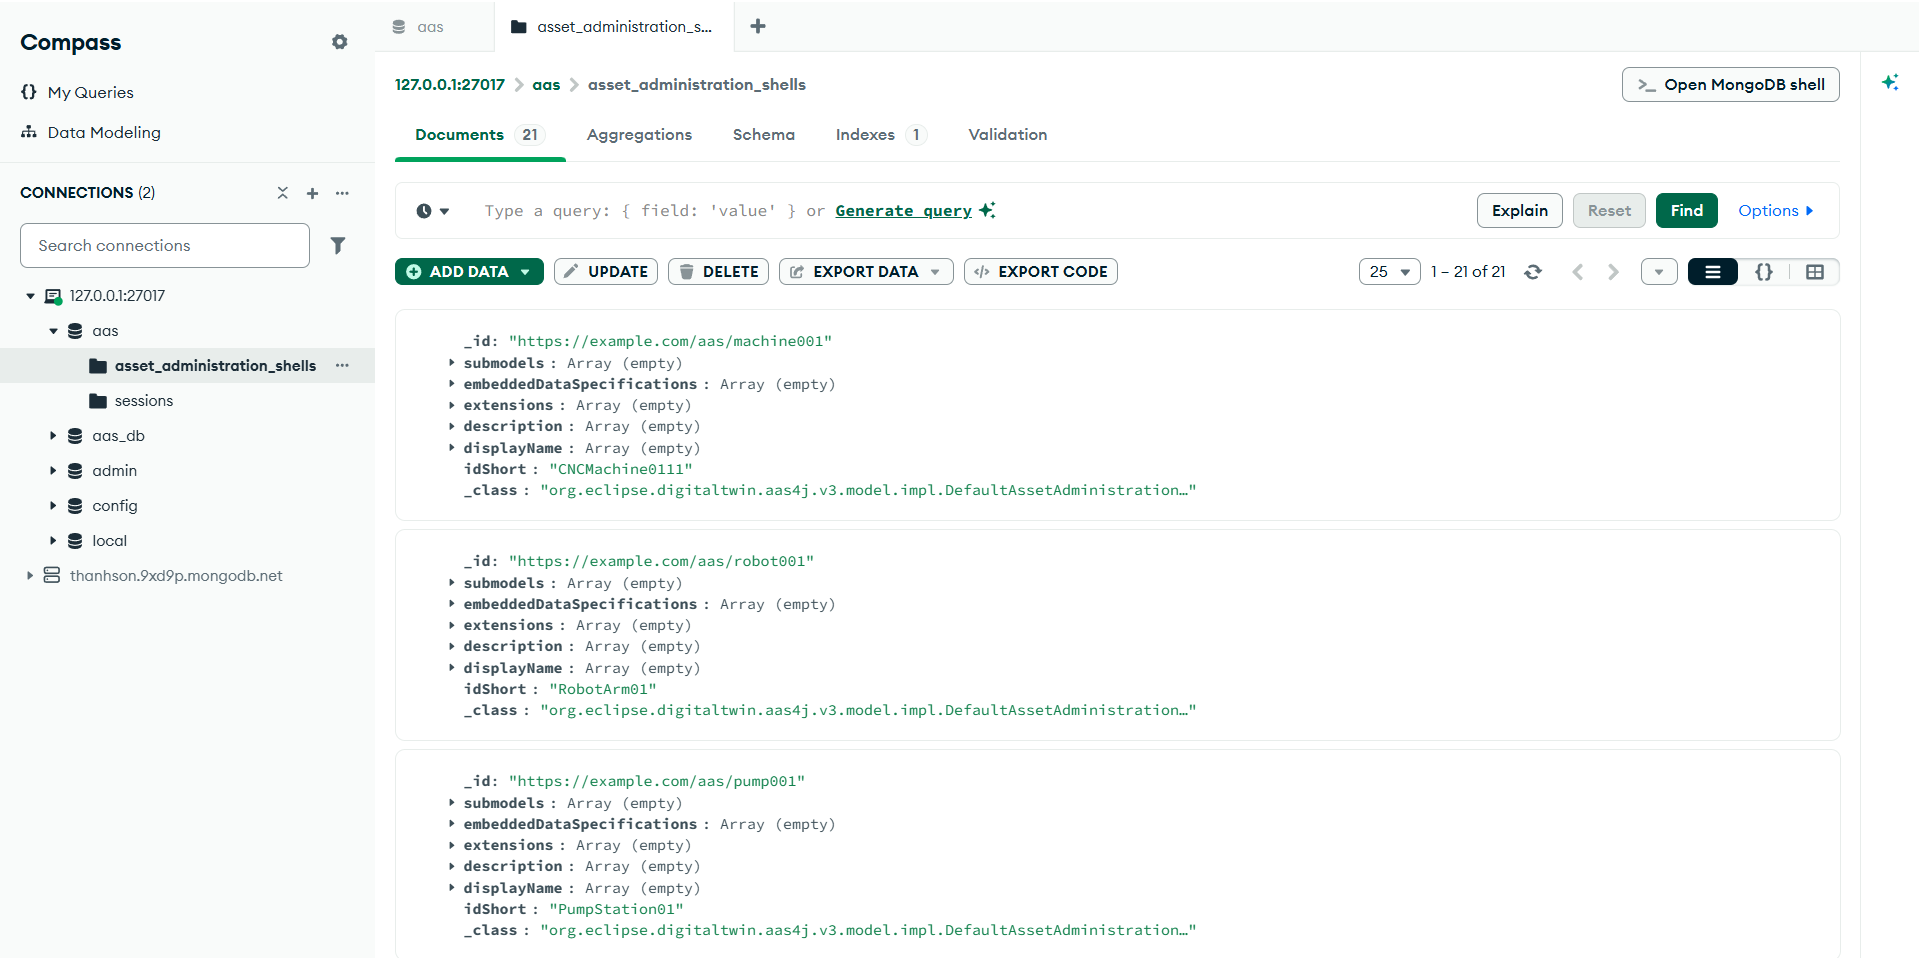
\includegraphics[width=\textwidth]{mongodb.png}
      \caption{Giao diện MongoDB Atlas hiển thị các Collection chứa dữ liệu AAS.}
      \label{fig:mongodb}
  \end{figure*}

	\item \textbf{Middleware:} Hệ thống sử dụng BaSyx DataBridge như một thành phần trung gian quan trọng để thực hiện khả năng liên thông giữa lớp vật lý (OT) và lớp ảo (IT). Thành phần này thu hẹp khoảng cách giao tiếp bằng cách chuyển đổi các thông điệp từ giao thức MQTT của các thiết bị Edge sang giao thức HTTP/REST mà máy chủ AAS yêu cầu. Quy trình xử lý dữ liệu tuân theo mô hình ETL: đầu tiên là trích xuất (Extract) dữ liệu từ MQTT Broker; tiếp theo là chuyển đổi (Transform) tải trọng thô thành định dạng JSON chuẩn hóa thông qua truy vấn JSONata; và cuối cùng là nạp (Load) dữ liệu vào máy chủ AAS bằng các yêu cầu HTTP PATCH.
\end{itemize}

\subsection{Quy trình Thực hiện}
\begin{itemize}
	\item \textbf{Cấu hình Hạ tầng:} Quá trình thiết lập hạ tầng kỹ thuật yêu cầu sự tinh chỉnh chính xác để đảm bảo khả năng tương tác thông suốt giữa giao diện người dùng và máy chủ dịch vụ backend. Tệp cấu hình \texttt{basyx-infra.yml} đã được điều chỉnh để trỏ đến địa chỉ \texttt{http://localhost:8081}. Việc thay đổi này giúp khắc phục các lỗi ``404 Not Found'' phát sinh khi UI cố gắng gọi các dịch vụ không tồn tại. Kết quả là máy chủ đã hoạt động ổn định như một Điểm truy cập duy nhất (Single Point of Access) tại địa chỉ \texttt{http://172.21.211.227:8081}.
	
  \begin{figure*}[h!]
      \centering
      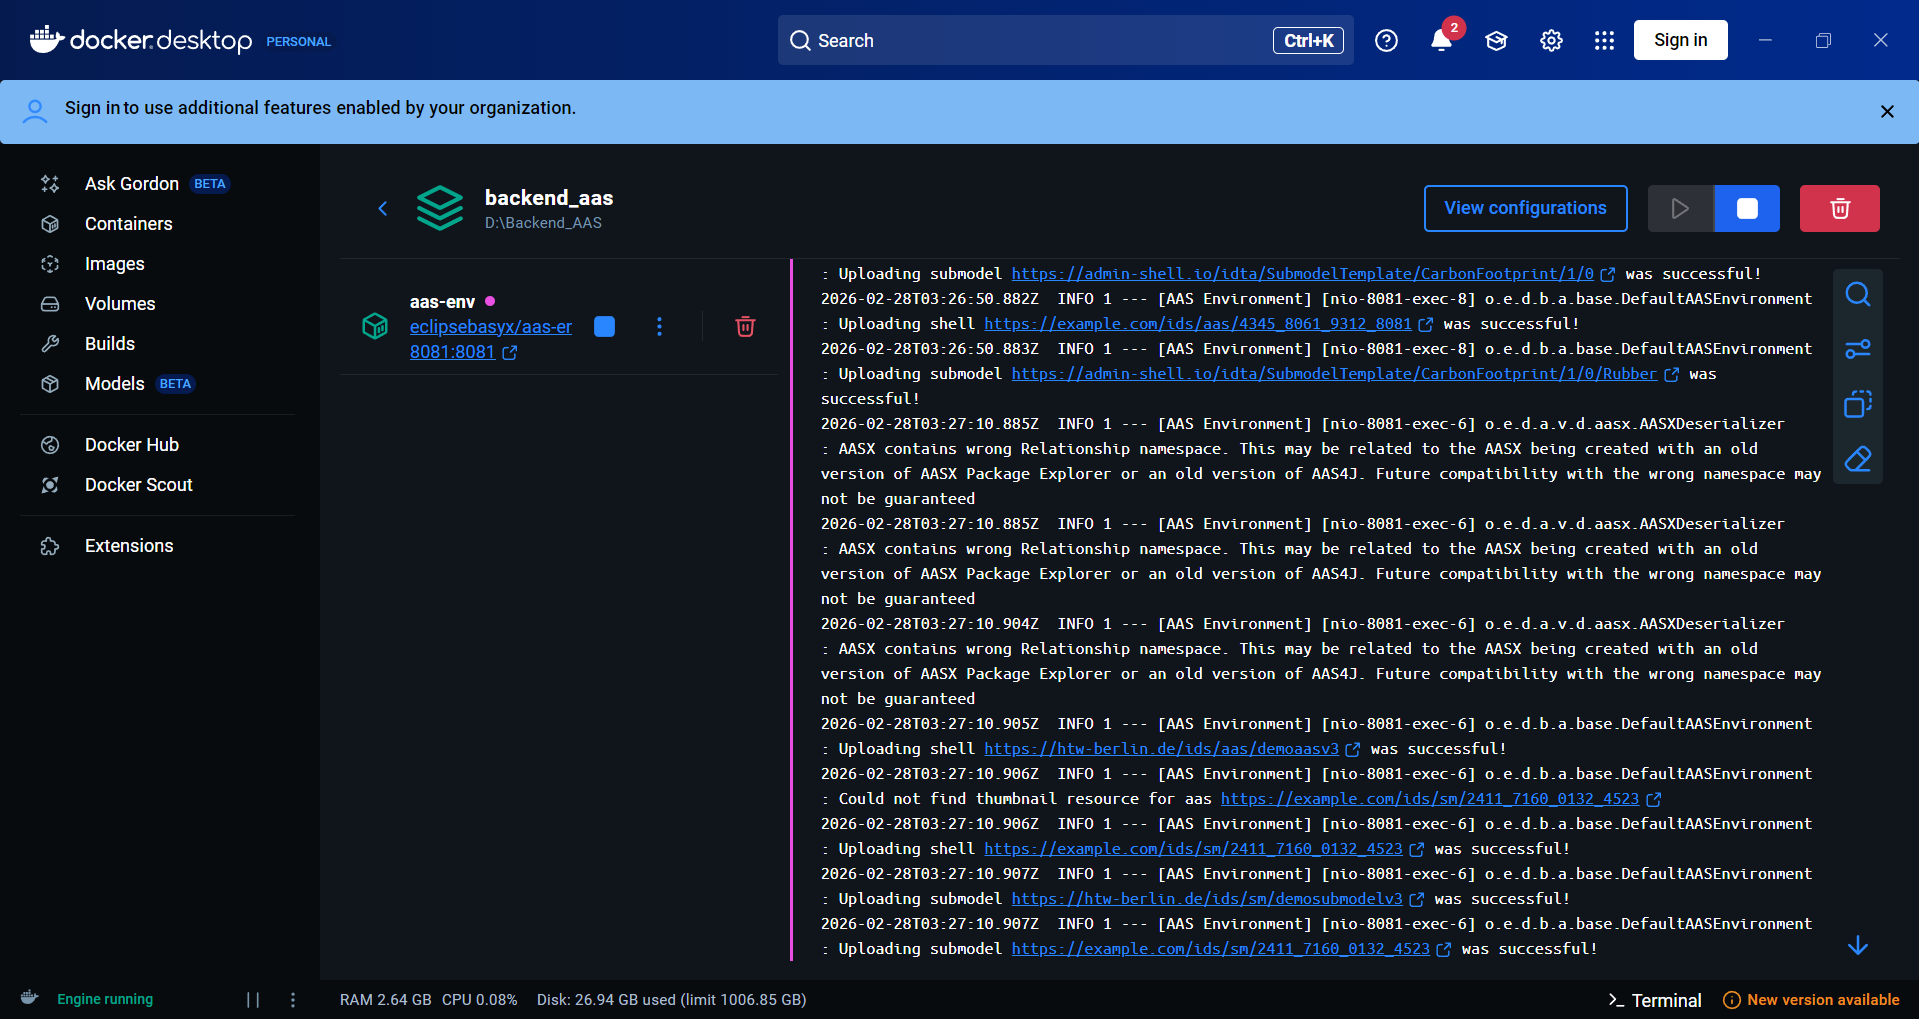
\includegraphics[width=\textwidth]{docker_container.png}
      \caption{Triển khai Docker Container cho BaSyx Backend Service trên cổng 8081.}
      \label{fig:docker}
  \end{figure*}

  \item \textbf{Định tuyến Dữ liệu:} Tệp cấu hình \texttt{routes.json} đã được xây dựng chi tiết nhằm điều phối quá trình ánh xạ thông tin thông qua BaSyx DataBridge. Hệ thống đăng ký và tiếp nhận dữ liệu đo lường thô từ MQTT Broker tại địa chỉ \texttt{tcp://mqtt-broker:1883} thông qua chủ đề \texttt{device/pc001/telemetry}. Các bộ chuyển đổi \texttt{jsonata} trích xuất chính xác các trường \texttt{\$.cpu\_usage} và \texttt{\$.ram\_usage}, sau đó đẩy tới các đích đến thông qua HTTP PATCH đến \texttt{CPUUsage/value} và \texttt{RAMUsage/value} thuộc Submodel \texttt{OperationalData}.
\end{itemize}

%% ================================================================
%%  PHẦN 3: KẾT QUẢ TRIỂN KHAI LOCAL
%% ================================================================
\section{Kết quả Triển khai trên Local}

\begin{itemize}
  \item \textbf{Giao diện Người dùng:} Hệ thống đã triển khai thành công giao diện Web UI dựa trên mã nguồn chính thức của Eclipse BaSyx, vận hành ổn định tại địa chỉ \texttt{http://localhost:3000}. Bố cục giao diện được thiết kế tối ưu với cấu trúc ba cột trực quan, cho phép người quản trị theo dõi toàn diện hệ thống bản sao số. Cột bên trái đóng vai trò là danh mục quản lý tập trung, hiển thị danh sách tất cả các AAS hiện có trên máy chủ. Cột giữa cung cấp cái nhìn chi tiết về cấu trúc phân cấp của tài sản được chọn. Cột bên phải là khu vực tương tác chuyên sâu, nơi hiển thị các giá trị đo lường, siêu dữ liệu và tích hợp các công cụ hình ảnh hóa.
  
  \begin{figure*}[h!]
      \centering
      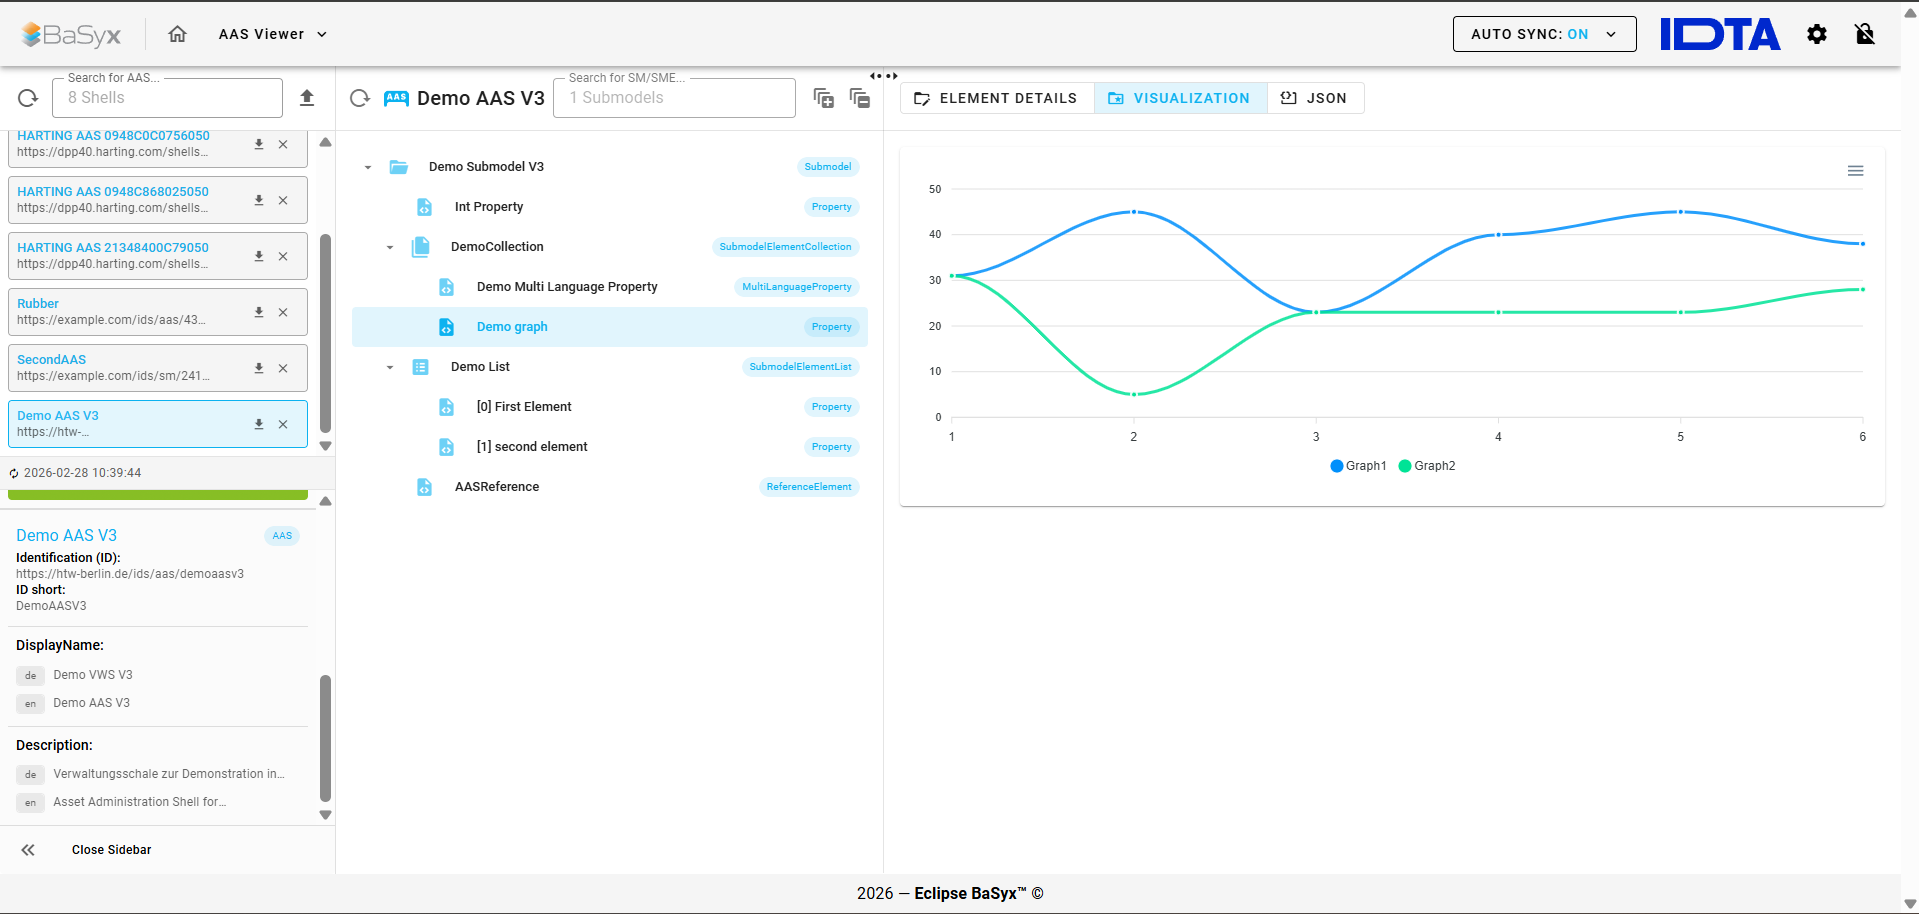
\includegraphics[width=\textwidth]{giaodiennguoidung.png}
      \caption{Giao diện người dùng Web UI với bố cục ba cột trực quan.}
      \label{fig:giaodien}
  \end{figure*}

  \item \textbf{Khả năng Quản lý:} Nền tảng hỗ trợ tải lên trực tiếp các tệp cấu hình tiêu chuẩn như \texttt{.aasx}, XML hoặc JSON. Nhóm đã tải lên thành công tệp \textit{Example V3.aasx}, cho phép hệ thống tự động phân tích và khởi tạo các thực thể số tương ứng trên Backend. Ngoài ra, giao diện còn cung cấp tab xem dữ liệu dưới định dạng JSON thô, giúp việc kiểm tra cấu trúc dữ liệu và gỡ lỗi API trở nên thuận tiện.

  \begin{figure*}[h!]
      \centering
      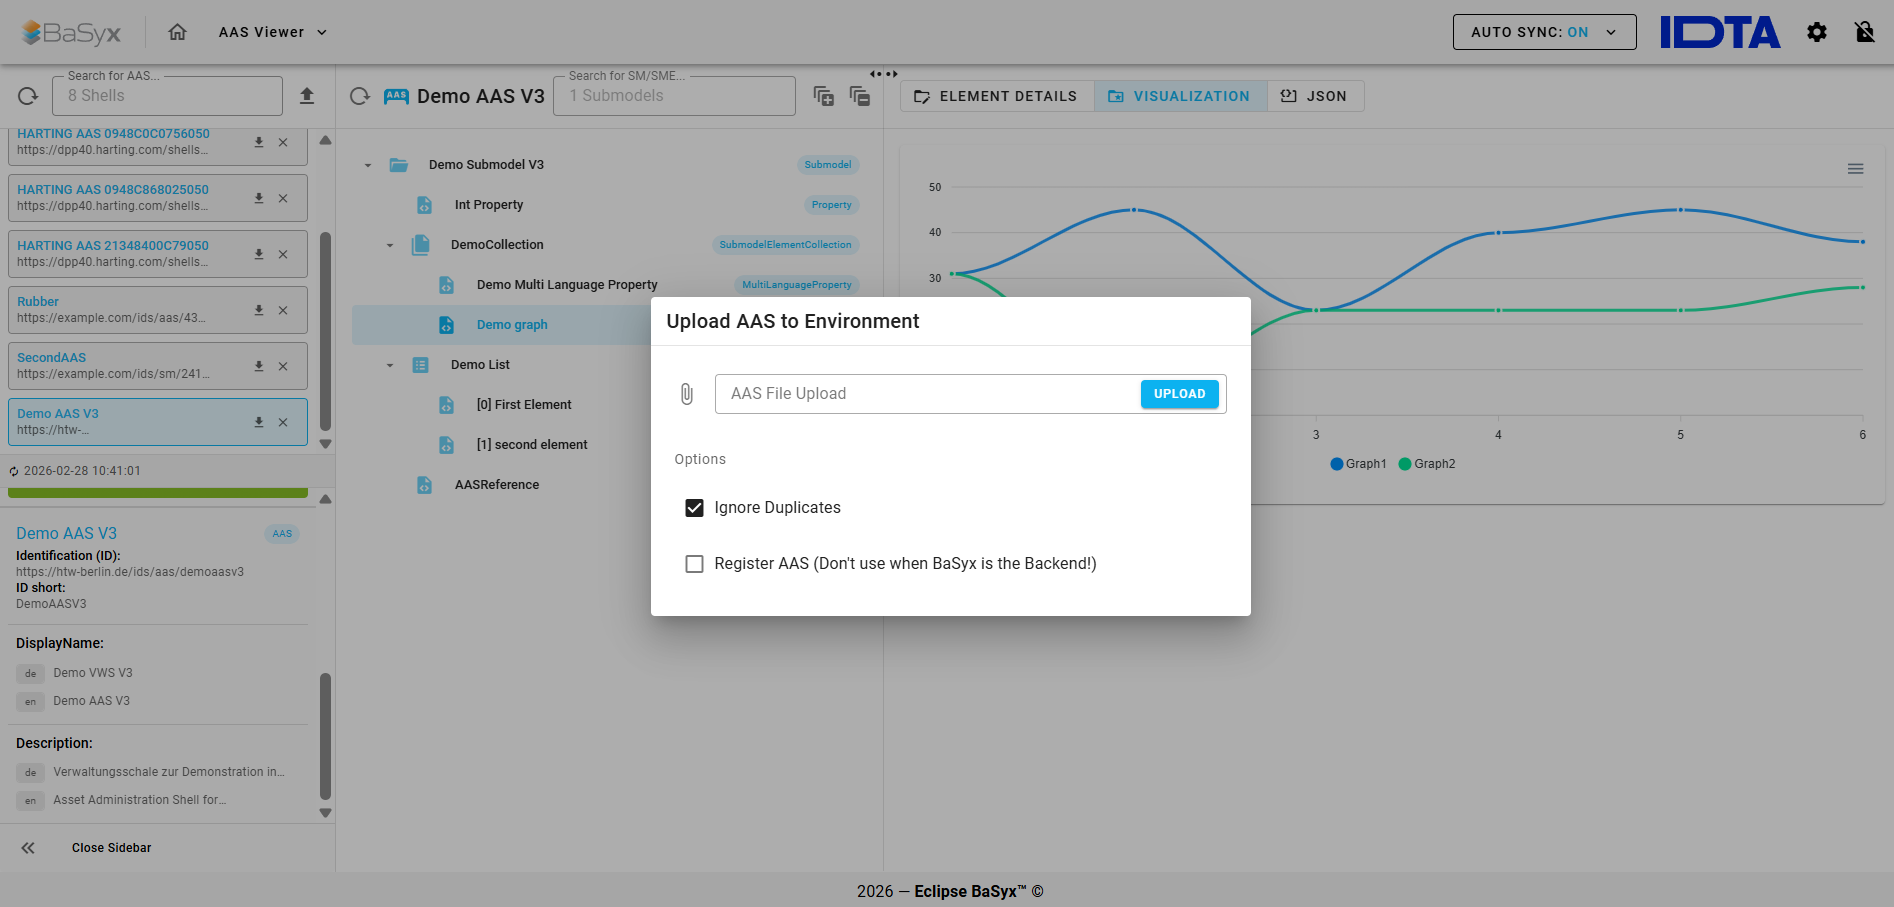
\includegraphics[width=\textwidth]{quanlytaisanso.png}
      \caption{Quản lý tài sản số thông qua việc tải lên tệp cấu hình và duyệt cấu trúc dữ liệu.}
      \label{fig:quanly}
  \end{figure*}

  \item \textbf{Tích hợp Dữ liệu Thời gian thực:} Dự án đã thiết lập thành công kịch bản giám sát máy trạm (Workstation). Thông qua script Python mô phỏng các node cảm biến, các thông số hiệu năng bao gồm CPU Usage và RAM Usage được truyền tải liên tục qua giao thức MQTT. Dữ liệu sau đó được BaSyx DataBridge xử lý theo mô hình ETL và cập nhật trực tiếp vào Submodel \textit{OperationalData}, phản ánh theo thời gian thực lên giao diện Web UI.
  
  \item \textbf{Hệ thống API:} Hệ thống cung cấp bộ API RESTful toàn diện, tuân thủ đặc tả OpenAPI của BaSyx. Các dịch vụ Repository cho phép thực hiện đầy đủ các thao tác CRUD trên Shells, Submodels và Concept Descriptions. Tính năng \textit{Value-Only representation} qua các endpoint \texttt{/\$value} giúp tối ưu hóa băng thông. Giao diện \texttt{invoke} cho phép kích hoạt các hàm vận hành từ xa (Operations), hỗ trợ cả chế độ đồng bộ và bất đồng bộ.

  \begin{figure*}[h!]
      \centering
      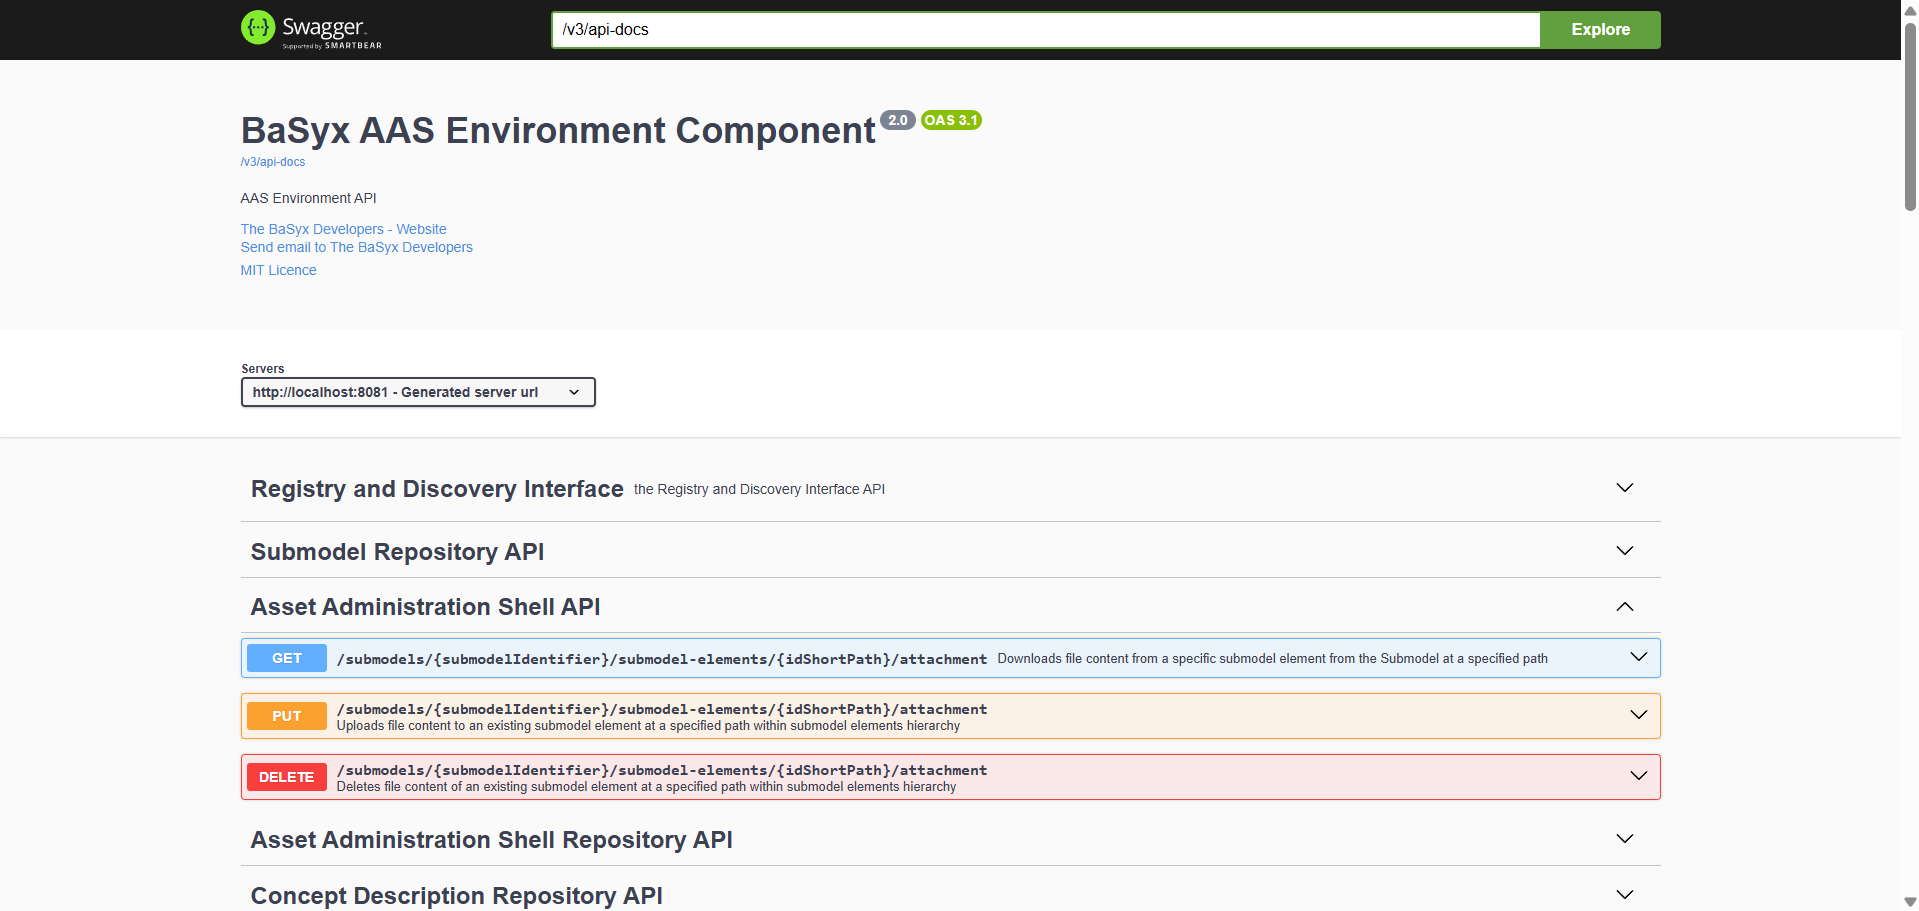
\includegraphics[width=\textwidth]{api_quanlytaisan.png}
      \caption{API quản lý tài sản số với các endpoint RESTful và chức năng invoke.}
      \label{fig:api}
  \end{figure*}
\end{itemize}

%% ================================================================
%%  PHẦN 4: THẢO LUẬN VỀ TRIỂN KHAI LOCAL
%% ================================================================
\section{Thảo luận}
\begin{itemize}
\item \textbf{Giải quyết Vấn đề Kỹ thuật:} Trong giai đoạn triển khai, nhóm đã đối mặt và xử lý triệt để hai thách thức kỹ thuật quan trọng. Thứ nhất là lỗi 404 Not Found, phát sinh do giao diện mặc định cố gắng gọi đến các dịch vụ Registry và Description chưa được kích hoạt. Vấn đề được khắc phục bằng cách điều chỉnh cấu hình hạ tầng. Thứ hai là lỗi CORS, xảy ra khi trình duyệt chặn các yêu cầu giữa cổng 3000 và cổng 8081. Giải pháp là bổ sung cấu hình \texttt{Basyx\_Cors\_Allowed-Origins=*} vào tệp Docker Compose.

\item \textbf{Ưu điểm của MongoDB:} Việc chuyển đổi sang MongoDB Atlas là bước tiến quan trọng nhằm giải quyết rủi ro mất mát dữ liệu khi sử dụng bộ nhớ tạm thời trong môi trường Docker. MongoDB được lựa chọn nhờ cấu trúc NoSQL hướng tài liệu, hoàn toàn tương đồng với định dạng JSON phân cấp của các đối tượng AAS, đồng thời có khả năng mở rộng ngang linh hoạt khi số lượng thiết bị tăng lên.

\item \textbf{Khả năng tương tác:} Tính liên thông được thể hiện qua cơ chế Serialization thông qua API \texttt{/serialization}, cho phép đóng gói toàn bộ mô hình Digital Twin vào một tệp tin duy nhất. Khả năng này hỗ trợ di chuyển và đồng bộ dữ liệu giữa các máy chủ AAS khác nhau trong môi trường sản xuất phân tán.
\end{itemize}

%% ================================================================
%%  PHẦN 5: TRIỂN KHAI LÊN SERVER
%% ================================================================
\section{Triển khai lên Server Công ty}

Sau khi hoàn thành giai đoạn phát triển và kiểm thử trên môi trường local, nhóm tiến hành triển khai hệ thống lên server thực tế của công ty Wisdom Software. Quá trình này bao gồm nhiều bước từ tiếp nhận thông tin server, thiết lập kết nối, thực hành deploy các dự án cơ bản cho đến nghiên cứu kiến trúc triển khai chuẩn.

\subsection{Tiếp nhận Thông tin Server}
Công ty Wisdom Software cung cấp cho nhóm một server chạy hệ điều hành \textbf{Ubuntu Linux} để phục vụ việc triển khai và vận hành các dự án. Thông tin server bao gồm:

\begin{table}[h!]
\centering
\small
\begin{tabular}{|l|l|}
\hline
\textbf{Thông số} & \textbf{Chi tiết} \\
\hline
Hệ điều hành & Ubuntu Linux \\
\hline
Nhà cung cấp & Wisdom Software \\
\hline
Phương thức kết nối & AnyDesk (Remote Desktop) \\
\hline
Mục đích & Deploy các dự án web, \\
 & Digital Twin, IoT \\
\hline
\end{tabular}
\caption{Thông tin Server được cung cấp bởi công ty}
\label{tab:server_info}
\end{table}

Server này đóng vai trò là môi trường staging/production cho các dự án của nhóm, cho phép kiểm tra khả năng vận hành thực tế của hệ thống trước khi đưa vào sử dụng chính thức.

\subsection{Cài đặt và Kết nối AnyDesk}
Để truy cập và quản lý server từ xa, nhóm sử dụng phần mềm \textbf{AnyDesk} -- một công cụ điều khiển máy tính từ xa (Remote Desktop) phổ biến. Quy trình thiết lập kết nối bao gồm:

\begin{enumerate}[noitemsep]
	\item \textbf{Cài đặt AnyDesk trên máy local:} Tải và cài đặt AnyDesk trên máy tính cá nhân (Windows).
	\item \textbf{Cài đặt AnyDesk trên server:} AnyDesk được cài đặt sẵn trên server Ubuntu Linux của công ty, với một ID kết nối cố định.
	\item \textbf{Thiết lập kết nối:} Nhập ID của server vào AnyDesk trên máy local, sử dụng mật khẩu được cung cấp bởi quản trị viên để xác thực.
	\item \textbf{Kiểm tra kết nối:} Sau khi kết nối thành công, nhóm có thể truy cập toàn bộ giao diện desktop của server Ubuntu, thao tác trực tiếp như đang ngồi trước máy chủ.
\end{enumerate}

Kết quả: Việc kết nối AnyDesk đã được thiết lập thành công, cho phép nhóm truy cập và quản lý server từ xa một cách ổn định. Giao diện desktop của server hiển thị đầy đủ với các thư mục dự án đã được triển khai, bao gồm: \texttt{webdeploy}, \texttt{deployment}, \texttt{Contructions}, \texttt{Microservices}, và các dự án khác.

\subsection{Thực hành Deploy các Dự án Cơ bản}
Trước khi triển khai dự án Digital Twin chính thức lên server, nhóm đã thực hiện các bài thực hành deploy nhiều dự án cơ bản để làm quen với quy trình triển khai trên môi trường Ubuntu Linux. Các dự án thực hành bao gồm:

\subsubsection{Dự án WTele}
\textbf{WTele} là một dự án web application thuộc hệ sinh thái của Wisdom Software. Dự án này đã được triển khai thử lên server nhằm kiểm tra khả năng hosting các ứng dụng web trên hạ tầng có sẵn.

\subsubsection{Dự án WCybersecurity-WebApp}
\textbf{WCybersecurity-WebApp} là ứng dụng web liên quan đến lĩnh vực an ninh mạng. Việc deploy dự án này giúp nhóm hiểu rõ hơn quy trình cấu hình các dịch vụ bảo mật và cổng mạng trên server Ubuntu.

\subsubsection{Dự án Master Construction3}
\textbf{Master Construction3} là dự án web thuộc lĩnh vực quản lý xây dựng. Việc deploy giúp nhóm thực hành cấu hình nhiều site chạy song song trên cùng một server, quản lý các cổng dịch vụ và xử lý conflict.

\subsubsection{Dự án pj\_python -- Bài thực hành Deploy với Docker}
Đây là dự án đặc biệt quan trọng trong quá trình học hỏi, được hướng dẫn trực tiếp bởi anh \textbf{Đặng Văn Phúc Nghĩa}. Dự án \texttt{pj\_python} là một project cơ bản bao gồm:

\begin{itemize}[noitemsep]
	\item \textbf{Frontend:} Giao diện web đơn giản phục vụ việc minh họa quy trình deploy.
	\item \textbf{Backend:} Xây dựng bằng Python với các API cơ bản.
	\item \textbf{Mục đích:} Là bài tập thực hành để học cách sử dụng Docker trong việc đóng gói và triển khai ứng dụng lên server.
\end{itemize}

Thông qua dự án này, nhóm đã nắm vững các kỹ năng quan trọng:
\begin{itemize}[noitemsep]
	\item Viết \texttt{Dockerfile} để đóng gói ứng dụng.
	\item Sử dụng \texttt{docker-compose.yml} để điều phối nhiều container.
	\item Build Docker Image và push lên Registry.
	\item Quản lý container lifecycle (start, stop, restart, logs).
\end{itemize}

\textbf{Lưu ý:} Tại giai đoạn này, các dự án được deploy chưa theo một cấu trúc kiến trúc chuẩn nào mà chủ yếu mang tính thử nghiệm và học hỏi. Việc thiếu một kiến trúc triển khai bài bản dẫn đến các vấn đề về quản lý tài nguyên, xung đột cổng và khó khăn trong việc mở rộng -- đây chính là động lực để nhóm tiến hành nghiên cứu chuyên sâu về kiến trúc triển khai chuẩn trong giai đoạn tiếp theo.

%% ================================================================
%%  PHẦN 6: NGHIÊN CỨU KIẾN TRÚC TRIỂN KHAI CHUẨN
%% ================================================================
\section{Nghiên cứu Kiến trúc Triển khai Chuẩn}

Sau giai đoạn thực hành deploy, nhóm nhận thấy rằng việc triển khai các ứng dụng -- đặc biệt là hệ thống Digital Twin phức tạp -- cần phải tuân theo một kiến trúc chuẩn nhằm đảm bảo hiệu suất, khả năng mở rộng và tính khả dụng cao. Hiện tại, nhóm đang tích cực nghiên cứu ba hướng chính: kiến trúc Container-based Microservices, cơ chế Load Balancing, và Resource Efficiency cho Digital Twin.

\subsection{Yêu cầu và Tiêu chuẩn khi Triển khai}
Dựa trên nghiên cứu tài liệu chuyên sâu, việc triển khai mã nguồn lên server trong các hệ thống IoT và Digital Twin cần tuân thủ các yêu cầu nghiêm ngặt:

\begin{itemize}
	\item \textbf{Hiệu quả tài nguyên và năng lượng:} Hệ thống phải tối ưu hóa việc tiêu thụ tài nguyên (CPU, RAM) và năng lượng, đặc biệt khi triển khai trên các thiết bị biên (Edge devices) có cấu hình hạn chế. Việc sử dụng ảo hóa dựa trên container (container-based virtualization) được khuyến nghị vì tiêu thụ ít tài nguyên hơn so với máy ảo truyền thống (VM).
	
	\item \textbf{Độ trễ thấp và băng thông:} Đối với các ứng dụng IoT và Digital Twin, yêu cầu quan trọng là độ trễ thấp (low latency) và băng thông cao để đảm bảo phản hồi thời gian thực giữa hệ thống ảo và thực thể vật lý.
	
	\item \textbf{Tính khả dụng cao (High Availability):} Hệ thống cần có khả năng tự phục hồi và mở rộng (scalability) theo nhu cầu mà không cần sự can thiệp của con người. Các cơ chế như Readiness Probe được yêu cầu để đảm bảo traffic không được gửi đến các pod chưa sẵn sàng xử lý.
	
	\item \textbf{Tiêu chuẩn giao thức:}
	\begin{itemize}[noitemsep]
		\item \textit{Giao thức ứng dụng:} Sử dụng CoAP hoặc MQTT cho các thiết bị IoT năng lượng thấp thay vì HTTP truyền thống. Đối với giao tiếp web/API, sử dụng RESTful API hoặc WebSocket.
		\item \textit{Đóng gói (Packaging):} Mã nguồn nên được đóng gói thành Docker Image (bản thiết kế bất biến) để đảm bảo tính nhất quán khi triển khai trên nhiều môi trường.
	\end{itemize}
\end{itemize}

\subsection{Kiến trúc Microservices dựa trên Container}
Các tài liệu đều hướng tới kiến trúc \textbf{Microservices} kết hợp với \textbf{Containerization} và \textbf{Orchestration}:

\begin{itemize}
	\item \textbf{Kiến trúc Microservices:} Thay vì mô hình Monolith (nguyên khối), mã nguồn nên được chia nhỏ thành các dịch vụ độc lập (microservices) để dễ dàng phát triển, triển khai và mở rộng. Mỗi dịch vụ chạy trong một container riêng biệt và giao tiếp qua giao thức mạng.

	\item \textbf{Mô hình ảo hóa Container (Docker):} Ứng dụng được đóng gói cùng các thư viện phụ thuộc vào trong các container nhẹ (lightweight). Container khởi động trong vài giây so với vài phút của VM và dễ dàng di chuyển giữa Cloud, Edge và thiết bị đầu cuối.

	\item \textbf{Container Orchestration:} Để quản lý các container, cần sử dụng các nền tảng điều phối như \textbf{Kubernetes} hoặc \textbf{Docker Swarm}. Trong Kubernetes, kiến trúc bao gồm Master Node (điều khiển) và Worker Nodes (nơi chạy các ứng dụng/pods). Ứng dụng được triển khai dưới dạng các Pod -- đơn vị nhỏ nhất chứa một hoặc nhiều container.

	\item \textbf{Kiến trúc Device-Edge-Cloud:} Đối với các hệ thống Digital Twin, kiến trúc phân tầng gồm Thiết bị (Device) -- Biên (Edge) -- Đám mây (Cloud) được đề xuất. Container cho phép di chuyển linh hoạt các dịch vụ mô phỏng giữa Edge và Cloud tùy theo nhu cầu xử lý.
\end{itemize}

\subsection{Nghiên cứu về Load Balancing}
Đây là hướng nghiên cứu trọng tâm hiện tại của nhóm nhằm chuẩn bị cho việc triển khai dự án Digital Twin lên server một cách chuyên nghiệp. Hai phương pháp chính được nghiên cứu:

\subsubsection{Phương án A: Load Balancing trong Kubernetes}
Trong Kubernetes, Load Balancing được thực hiện thông qua đối tượng \textbf{Service} để phân phối traffic đến các Pod:

\begin{itemize}[noitemsep]
	\item \textbf{ClusterIP:} Cấp IP nội bộ, chỉ truy cập được từ bên trong cluster.
	\item \textbf{NodePort:} Mở một cổng cụ thể trên mỗi Node để truy cập từ bên ngoài.
	\item \textbf{LoadBalancer:} Sử dụng bộ cân bằng tải của nhà cung cấp đám mây để điều hướng traffic vào NodePort.
\end{itemize}

Bên cạnh đó, \textbf{Horizontal Pod Autoscaler (HPA)} cho phép tự động tăng/giảm số lượng Pod dựa trên tải (CPU/RAM hoặc custom metrics). Nhóm nghiên cứu hai loại metric:
\begin{itemize}[noitemsep]
	\item \textit{Resource Metrics (Mặc định):} Dựa trên CPU/RAM, phù hợp với tải ổn định.
	\item \textit{Custom Metrics:} Sử dụng Prometheus để đo chỉ số tùy chỉnh như request rate, giúp phản ứng nhanh hơn với đợt tăng tải đột biến (flash crowds).
\end{itemize}

\subsubsection{Phương án B: Load Balancing với Nginx và Tailscale VPN}
Một phương án chi phí thấp, phù hợp với quy mô nhỏ/vừa, sử dụng \textbf{Nginx} làm Public Edge server kết hợp với \textbf{Tailscale} (VPN dựa trên WireGuard):

\begin{itemize}
	\item \textbf{Kiến trúc:} Một máy chủ Edge có IP công cộng chạy Nginx nhận traffic từ Internet, sau đó reverse proxy qua mạng Tailscale đến các server hạ nguồn.
	\item \textbf{Cơ chế Failover:} Cấu hình Nginx với khối \texttt{upstream} định nghĩa server chính và server backup. Nếu server chính lỗi, Nginx tự động chuyển sang server backup qua IP Tailscale.
	\item \textbf{Bảo mật:} Traffic giữa Edge và các server ứng dụng được mã hóa đầu cuối (E2E) bởi Tailscale. Các server ứng dụng không cần mở cổng ra Internet công cộng.
\end{itemize}

Ví dụ cấu hình Nginx:
\begin{lstlisting}[language=bash, caption={Cấu hình upstream trong Nginx}]
upstream backend_pool {
    server 100.64.A.A:8081;  # Primary
    server 100.64.B.B:8081 backup; # Backup
    keepalive 32;
}

server {
    listen 443 ssl;
    server_name dt.wisdom.vn;
    
    location / {
        proxy_pass http://backend_pool;
        proxy_set_header Host $host;
        proxy_set_header X-Real-IP
          $remote_addr;
    }
}
\end{lstlisting}

\subsection{Nghiên cứu về Resource Efficiency cho Digital Twin}
Nhóm đang nghiên cứu các giải pháp tối ưu hóa tài nguyên khi triển khai hệ thống Digital Twin trên server:

\begin{itemize}
	\item \textbf{Lightweight Container Image:} Sử dụng các base image nhẹ như Alpine Linux để giảm dung lượng đĩa (trung bình giảm 70\% kích thước image), tăng tốc độ triển khai và giảm tiêu thụ tài nguyên.
	
	\item \textbf{Readiness Probe và Liveness Probe:} Cấu hình các tính năng health check trong Kubernetes để đảm bảo traffic chỉ được gửi đến các Pod đã sẵn sàng xử lý, giảm tỷ lệ lỗi request khi đang autoscaling.
	
	\item \textbf{Tối ưu hóa Giao thức:} Sử dụng CoAP thay vì HTTP cho các thiết bị IoT năng lượng thấp, và MQTT cho truyền dữ liệu cảm biến -- phù hợp với mô hình publish/subscribe và tiêu thụ ít tài nguyên mạng.
\end{itemize}

\subsection{Kế hoạch Triển khai Tiếp theo}
Dựa trên kết quả nghiên cứu, nhóm đề xuất kế hoạch triển khai dự án Digital Twin lên server theo các bước sau:

\begin{enumerate}
	\item \textbf{Bước 1 -- Containerization:} Đóng gói toàn bộ các thành phần (Frontend, Backend, MongoDB, DataBridge) thành các Docker Image riêng biệt với \texttt{Dockerfile} được tối ưu hóa.
	
	\item \textbf{Bước 2 -- Docker Compose:} Thiết lập tệp \texttt{docker-compose.yml} hoàn chỉnh để điều phối tất cả các container, đảm bảo mạng nội bộ (overlay network) và quản lý volumes cho dữ liệu bền vững.
	
	\item \textbf{Bước 3 -- Cấu hình Nginx Reverse Proxy:} Thiết lập Nginx làm reverse proxy phía trước, xử lý HTTPS (SSL/TLS), cân bằng tải và cacheable responses.
	
	\item \textbf{Bước 4 -- Load Balancing:} Áp dụng phương án Load Balancing phù hợp với quy mô hiện tại (Nginx + Tailscale cho giai đoạn đầu, Kubernetes cho giai đoạn mở rộng).
	
	\item \textbf{Bước 5 -- Monitoring và Alerting:} Tích hợp các công cụ giám sát như Prometheus và Grafana để theo dõi sức khỏe hệ thống, cảnh báo khi tài nguyên vượt ngưỡng.
\end{enumerate}

%% ================================================================
%%  PHẦN 7: KẾT LUẬN
%% ================================================================
\section{Kết luận}
Dự án ``Hybrid-Digital Twin Platform'' đã hoàn thành thành công ba giai đoạn quan trọng:

\begin{enumerate}
	\item \textbf{Giai đoạn Nghiên cứu:} Nhóm đã nghiên cứu và nắm vững ý tưởng về số hóa thiết bị thông qua công nghệ Digital Twin, hiểu rõ cơ chế vận hành của Asset Administration Shell (AAS) và các tiêu chuẩn quốc tế IEC 63278 và ISO 23247-2.
	
	\item \textbf{Giai đoạn Triển khai Local:} Hệ thống đã được triển khai thành công trên môi trường local với đầy đủ các thành phần: giao diện React hoạt động tại cổng 3000, backend Docker cung cấp API RESTful tại cổng 8081, cơ sở dữ liệu MongoDB Atlas đảm bảo lưu trữ bền vững, và BaSyx DataBridge thực hiện truyền dữ liệu thời gian thực từ MQTT đến bản sao số.
	
	\item \textbf{Giai đoạn Triển khai Server:} Nhóm đã thiết lập kết nối thành công với server công ty thông qua AnyDesk, thực hành deploy nhiều dự án cơ bản (WTele, WCybersecurity-WebApp, Master Construction3, pj\_python) và hiện đang nghiên cứu chuyên sâu về kiến trúc Load Balancing, Container Orchestration và Resource Efficiency để chuẩn bị triển khai dự án Digital Twin lên server theo đúng chuẩn kiến trúc hiện đại.
\end{enumerate}

Hướng phát triển tiếp theo tập trung vào việc hoàn thiện kiến trúc triển khai chuẩn Microservices trên server Ubuntu Linux, tích hợp cơ chế Load Balancing với Nginx hoặc Kubernetes, và thực hiện tự động hóa quy trình CI/CD để đảm bảo hệ thống Digital Twin vận hành liên tục, ổn định và có khả năng mở rộng trong môi trường sản xuất thực tế.

%% ================================================================
%%  LỜI CẢM ƠN VÀ TÀI LIỆU THAM KHẢO
%% ================================================================
\twocolumn[
	\begin{@twocolumnfalse}
		\section*{Lời cảm ơn}
		Báo cáo này được thực hiện bởi đội ngũ kỹ thuật tại Wisdom Software. Nhóm dự án bao gồm: Thái Đặng Phương Nam (Người báo cáo chính), Nguyễn Lê Thanh Phong, và Huỳnh Thanh Sơn. Nhóm xin gửi lời cảm ơn đặc biệt đến anh Đặng Văn Phúc Nghĩa đã hướng dẫn trực tiếp về quy trình deploy với Docker trên server. Nghiên cứu được hoàn thành vào tháng 03 năm 2026 tại TP. Hồ Chí Minh.
		\vspace{1.5em}
		\printbibliography
	\end{@twocolumnfalse}
]

\end{document}
